\section{Results and Discussion}
\label{sec:results}
All experiments used an epsilon value of 1e-10 as the difference between iterative computations of the probability distributions. Unfortunately, the ranking results are inherently difficult to quantify, especially without first defining an appropriate loss/cost function that captures exactly what and how one would measure `importance'. Once these results are scaled up to integrate the 20,000 datasets indexed in the DataRank prototype, users can be brought in for testing. However, before that occurs we conduct a solely qualitative evaluation, like that used by Corank and Multirank. We differ in that we try to examine quantities captured by the network structure, while other evaluations rely on agreement between `expert judges' that numerically assess authors based on knowledge of their research domain community.

\paragraph{Paper Ranking}\footnote{Italicized PMID indicate original paper of data series}
Individual ranking of papers took 151 iterations to converge in 12.45 seconds. As can be seen from Table~\ref{tab:paper_rank}, there is little variability between the top 15 papers when ranked individually and coranked. The six original papers which were cited more than hundreds of times appear in the top nine rankings. It is not entirely clear why PMID 17069663 and 16417655 are so highly ranked because they have low cited by counts, but it should be noted that they do cite the top ranked original paper.

    \begin{table}[h]
    \resizebox{\columnwidth}{!}{
    \begin{tabular}{|c|cc|cc|}
    \hline
    \textbf{Ranking} & \textbf{PMID (Indiv.)} & \textbf{\# Cited By} & \textbf{PMID (Corank)} & \textbf{\# Cited By} \\ \hline
    1 & \textit{12297621} & 212 & \textit{12297621} & 212 \\
    2 & \textit{16273092} & 418 & \textit{16273092} & 418 \\
    3 & \textit{15193263} & 129 & \textit{15193263} & 129 \\
    4 & \textit{16141321} & 337 & \textit{16141321} & 337 \\
    5 & \textit{16478745} & 342 & \textit{16478745} & 342 \\
    6 & 17069663 & 12 & 17157791 & 519 \\
    7 & 17157791 & 519 & 16643655 & 254 \\
    8 & 16643655 & 254 & \textit{16280042} & 203 \\
    9 & \textit{16280042} & 203 & 15034139 & 54 \\
    10 & 15034139 & 54 & 18948947 & 284 \\
    11 & 18948947 & 284 & 18443585 & 297 \\
    12 & 16585533 & 82 & 16585533 & 82 \\
    13 & 18443585 & 297 & 17493263 & 210 \\
    14 & 16417655 & 20 & 16417655 & 20 \\
    15 & 17493263 & 210 & 17069663 & 12 \\ \hline
    \end{tabular}}
    \caption{Paper Ranking: Individual vs. Corank}
    \label{tab:paper_rank}
    \end{table}

Table~\ref{tab:paper_ranking_analysis} displays the rankings for the nine original papers that appeared in the top 100 journals, and shows that there is little difference between individual and coranking. As an aside, we include the number of samples for each dataset. We also display the cumulative number of publications within our corpus by the authors of the dataset. We admit it is difficult to evaluate the output of the paper rankings. Ranking papers more effectly would require more processing, perhaps first running a topic model and then ranking within a research area. Fortunately, we are more interested in the results of the author ranking for augmenting the DataRank prototype.

    \begin{table}[h]
    \resizebox{\columnwidth}{!}{
    \begin{tabular}{c|c|ccc|}
    \cline{2-5}
    {\color[HTML]{9B9B9B} {\bf \# Data Samples}} & {\bf Original PMID} & {\bf Indiv. Rank} & {\bf Corank} & {\bf Cited By} \\ \cline{2-5} 
    {\color[HTML]{9B9B9B} 100} & 12297621 & 1 & 1 & 212 \\
    {\color[HTML]{9B9B9B} 158} & 16273092 & 2 & 2 & 418 \\
    {\color[HTML]{9B9B9B} 60} & 15193263 & 3 & 3 & 129 \\
    {\color[HTML]{9B9B9B} 502} & 16141321 & 4 & 4 & 337 \\
    {\color[HTML]{9B9B9B} 189} & 16478745 & 5 & 5 & 342 \\
    {\color[HTML]{9B9B9B} 318} & 16280042 & 9 & 8 & 203 \\
    {\color[HTML]{9B9B9B} 126} & 16626501 & 20 & 20 & 36 \\
    {\color[HTML]{9B9B9B} 180} & 16505412 & 25 & 26 & 37 \\
    {\color[HTML]{9B9B9B} 17} & 16849584 & 44 & 51 & 42 \\ \cline{2-5} 
    \end{tabular}}
    \caption{Paper Ranking Analysis}
    \label{tab:paper_ranking_analysis}
    \end{table}

    % \begin{table}[h]
    % \resizebox{\columnwidth}{!}{
    % \begin{tabular}{|c|cccc|}
    % \hline
    % \textbf{Original PMID} & \textbf{Individual Rank} & \textbf{Corank} & \textbf{\# Cited By} & \textbf{\# Papers for Authors} \\ \hline
    % 12297621 & 1 & 1 & 212 & 55 \\
    % 16273092 & 2 & 2 & 418 & 31 \\
    % 15193263 & 3 & 3 & 129 & 14 \\
    % 16141321 & 4 & 4 & 337 & 13 \\
    % 16478745 & 5 & 5 & 342 & 31 \\
    % 16280042 & 9 & 8 & 203 & 11 \\
    % 16626501 & 20 & 20 & 36 & 14 \\
    % 16505412 & 25 & 26 & 37 & 15 \\
    % 16849584 & 44 & 51 & 42 & 20 \\ \hline
    % \end{tabular}}
    % \caption{Paper Ranking Analysis}
    % \label{tab:paper_ranking_analysis}
    % \end{table}


\paragraph{Individual Author Ranking} \footnote{Italicized names indicate authors of original paper of data series}
Individual author ranking took 32 iterations to converge in 15.66 sec. From Table~\ref{tab:author_indiv}, one can observe the general trend that authors with many collaborations are highly individually ranked. This trend is not a surprise because of how individual ranking works --- by using the structure of the collaboration network. An author with more links and stronger links simply has higher probability of being visited in a random walk. As an example, we attempt to explain why Nevins (rank 8) ranks higher than Pollack (rank 9). Both have the same number of publications; Nevins has fewer coauthors but his coauthor links are stronger with a sum of 48 links (vs. a sum of 45 links for Pollack). Individual ranking only takes place on the author graph, so the number of papers should not affect its outcome. However, having many publications and having many coauthors usually go hand in hand. Only three of the top 15 authors, who also happen to be highly coranked, are associated with the original papers. 

    \begin{table}[h]
    \resizebox{\columnwidth}{!}{
    \begin{tabular}{|c|ccccc|}
    \hline
    \textbf{Indiv. Ranking} & \textbf{Author} & \textbf{\# Coauthors} & \textbf{\# Papers} & \textbf{Rank in Corank} & \textbf{Rank in Multirank} \\ \hline
    1 & Creighton, Chad J & 44 & 28 & 39 & 66 \\
    2 & \textit{Perou, Charles M} & 43 & 28 & 1 & 3 \\
    3 & Zhang, Wei & 22 & 18 & 292 & 500+ \\
    4 & Pusztai, Lajos & 36 & 21 & 63 & 318 \\
    5 & Teschendorff, Andrew E & 30 & 21 & 43 & 7 \\
    6 & Haibe-Kains, Benjamin & 33 & 22 & 34 & 500+ \\
    7 & Massague, Joan & 21 & 19 & 10 & 74 \\
    8 & \textit{Nevins, Joseph R} & 24 & 19 & 5 & 198 \\
    9 & \textit{Pollack, Jonathan R} & 25 & 19 & 2 & 2 \\
    10 & Chinnaiyan, Arul M & 23 & 20 & 128 & 500+ \\
    11 & Arteaga, Carlos L & 23 & 21 & 211 & 500+ \\
    12 & Katzenellenbogen, Benita S & 29 & 16 & 82 & 16 \\
    13 & Liu, Edison T & 23 & 13 & 31 & 103 \\
    14 & Caldas, Carlos & 31 & 18 & 47 & 23 \\
    15 & Weinberg, Robert A & 18 & 17 & 21 & 98 \\ \hline
    \end{tabular}}
    \caption{Top Authors by Individual Ranking}
    \label{tab:author_indiv}
    \end{table}


\paragraph{Author Corank}
Coranking (both papers and authors) took 74 iterations to converge in 11.58 sec. Already we see an improvement to individual ranking with eleven of the top fifteen being authors associated with the original papers. We expect authors with many publications and many coauthors to be ranked highly, which is generally the case, but there are some authors with few papers that appear highly ranked. We suspect this is because they are mostly original authors who are coauthored with an author of high rank or connected to papers with a high number of citations. For example, authors Ma, Yao, Sorlie (ranked 6, 13, 14, respectively) all have less than 5 publications and less than or equal to 10 coauthors but they are original authors and strongly connected to Perou, Pollack, Brown, and Nevins (ranked 1, 2, 3, 5, respectively). Authors Bergh and Miller (ranked 9 and 12) also have few paper and coauthor counts, but they are the authors of highly individually ranked PMID 161413321 (337 citations). Seventh ranked You is not an original author but he has coauthored multiple times with highly ranked Nevins and Yao. Tenth ranked Massague is also not an original author, but her total citation count of 466 is almost double than what would be expected based on her publication number and the mean PMID cited by count of 13. 

    \begin{table}[h]
    \resizebox{\columnwidth}{!}{
    \begin{tabular}{|c|ccccc|}
    \hline
    \textbf{Corank} & \textbf{Author} & \textbf{\# Papers} & \textbf{\# Coauthors} & \textbf{Rank Individually} & \textbf{Rank in Multirank} \\ \hline
    1 & \textit{Perou, Charles M} & 28 & 43 & 2 & 3 \\
    2 & \textit{Pollack, Jonathan R} & 19 & 25 & 9 & 2 \\
    3 & \textit{Brown, Patrick O} & 6 & 8 & 381 & 100 \\
    4 & \textit{Sgroi, Dennis C} & 11 & 25 & 29 & 30 \\
    5 & \textit{Nevins, Joseph R} & 19 & 24 & 8 & 198 \\
    6 & \textit{Ma, Xiao-Jun} & 4 & 6 & 413 & 41 \\
    7 & You, Lingchong & 8 & 5 & 119 & 500+ \\
    8 & \textit{Chang, Jeffrey T} & 12 & 19 & 51 & 316 \\
    9 & \textit{Bergh, Jonas} & 4 & 8 & 917 & 1 \\
    10 & Massague, Joan & 19 & 21 & 7 & 74 \\
    11 & Parker, Joel S & 14 & 26 & 53 & 6 \\
    12 & \textit{Miller, Lance D} & 7 & 14 & 190 & 12 \\
    13 & \textit{Yao, Guang} & 5 & 7 & 1229 & 500+ \\
    14 & \textit{Sorlie, Therese} & 5 & 10 & 1474 & 43 \\
    15 & Lam, Wan L & 22 & 21 & 17 & 58 \\ \hline
    \end{tabular}}
    \caption{Top Authors by Corank}
    \label{tab:author_corank}
    \end{table}



\paragraph{Multirank}
Multiranking authors with journal relations took 21 iterations to converge in 78.2 sec. Eleven of the top fifteen are original authors, but they are not the same eleven that appear for corank; however, there is an overlap of five authors, four of which are original authors. Interestingly, the bottom half of Table~\ref{tab:multi} have few papers, and are very lowly ranked individually, but the papers they've published are highly cited, published in the top journals, and thus they make up a strong portion of the overall network. 

Chin (ranked 10) and Bocanegra (ranked 13) seem like outliers as they are neither original authors nor have many papers and coauthors. However, one of the two papers authored by Chin has a 519 cited by count, which makes it the top cited paper. Bocanegra coauthored both papers with 2nd ranked Pollack, and her papers cite three of the original papers.

    \begin{table}[h]
    \resizebox{\columnwidth}{!}{
    \begin{tabular}{|c|ccccc|}
    \hline
    \textbf{Multirank} & \textbf{Author} & \textbf{\# Papers} & \textbf{\# Coauthors} & \textbf{Rank in Corank} & \textbf{Rank Individually} \\ \hline
    1 & \textit{Bergh, Jonas} & 4 & 8 & 9 & 917 \\
    2 & \textit{Pollack, Jonathan R} & 19 & 25 & 2 & 9 \\
    3 & \textit{Perou, Charles M} & 28 & 43 & 1 & 2 \\
    4 & \textit{Sotiriou, Christos} & 15 & 25 & 16 & 48 \\
    5 & \textit{Pawitan, Yudi} & 8 & 17 & 19 & 84 \\
    6 & Parker, Joel S & 14 & 26 & 11 & 53 \\
    7 & Teschendorff, Andrew E & 21 & 30 & 43 & 5 \\
    8 & \textit{Delorenzi, Mauro} & 8 & 11 & 23 & 195 \\
    9 & \textit{Wirapati, Pratyaksha} & 5 & 12 & 50 & 1266 \\
    10 & Chin, Koei & 2 & 4 & 70 & 7421 \\
    11 & \textit{Bjohle, Judith} & 1 & 2 & 79 & 9435 \\
    12 & \textit{Miller, Lance D} & 7 & 14 & 12 & 190 \\
    13 & Bocanegra, Melanie & 2 & 5 & 269 & 8421 \\
    14 & \textit{George, Joshy} & 4 & 7 & 34 & 2281 \\
    15 & \textit{Smeds, Johanna} & 1 & 3 & 80 & 10788 \\ \hline
    \end{tabular}}
    \caption{Top Authors by Multirank}
    \label{tab:multi}
    \end{table}

Ranking of the top ten journals seen in Table~\ref{tab:journal} suggest that the general trend is to rank by number of papers published within a journal. Journals with many publications inherently leads to more authors, and probably with authors of higher influence within the network. The lower ranking for journal 5 and 6 which both published a paper connected to an original dataset may suggest that the original paper does not have a great influence on the journal rank. This may be because those original papers are not as highly cited as other papers. Regardless, we note that the original nine papers appear in the top 27 journals.

    \begin{table}[h]
    \resizebox{\columnwidth}{!}{
    \begin{tabular}{|c|lcc|}
    \hline
     & \multicolumn{1}{c}{{\bf Journal}} & {\bf \# Papers} & {\bf \# Originals} \\ \hline
    {\bf 1} & PloS one & 1692 & --- \\
    {\bf 2} & Breast cancer research : BCR & 483 & 2 \\
    {\bf 3} & Proceedings of the National Academy of Sciences of the USA & 419 & 2 \\
    {\bf 4} & BMC bioinformatics & 369 & --- \\
    {\bf 5} & Cancer research & 422 & 1 \\
    {\bf 6} & Cancer cell & 136 & 1 \\
    {\bf 7} & Bioinformatics (Oxford, England) & 174 & --- \\
    {\bf 8} & BMC genomics & 289 & --- \\
    {\bf 9} & Genome research & 130 & --- \\
    {\bf 10} & The Journal of clinical investigation & 156 & --- \\ \hline
    \end{tabular}}
    \caption{Top Multiranked Journals}
    \label{tab:journal}
    \end{table}


    \begin{figure}[t!]
        \centering
        \subfigure[Author Multirank]{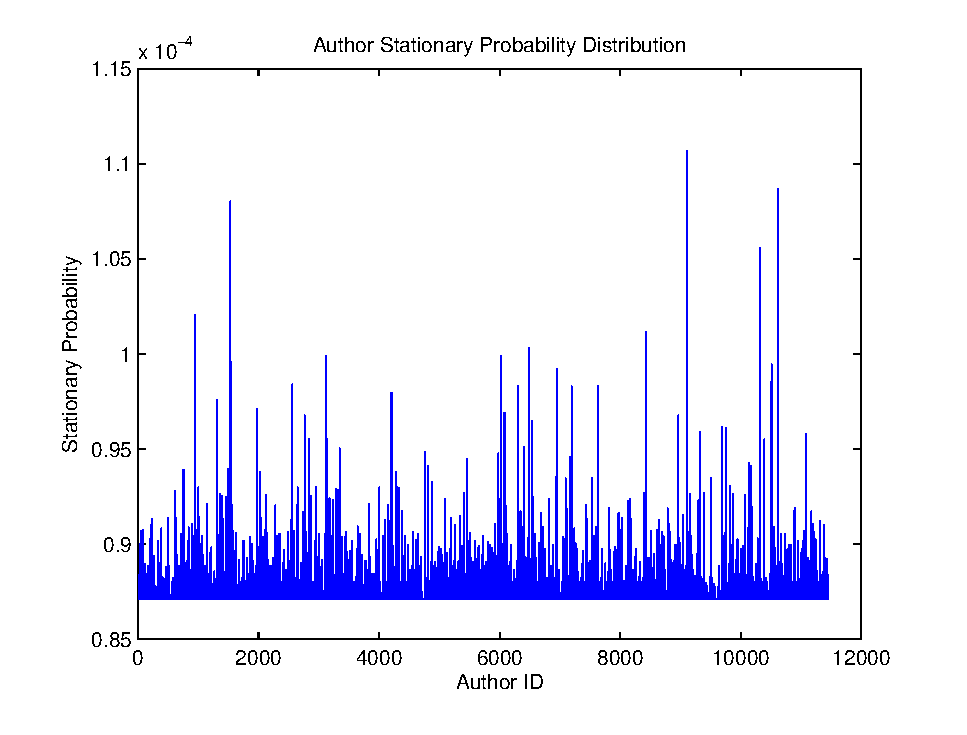
\includegraphics[width=\columnwidth]{author_dist.eps}}
        \subfigure[Journal Multirank]{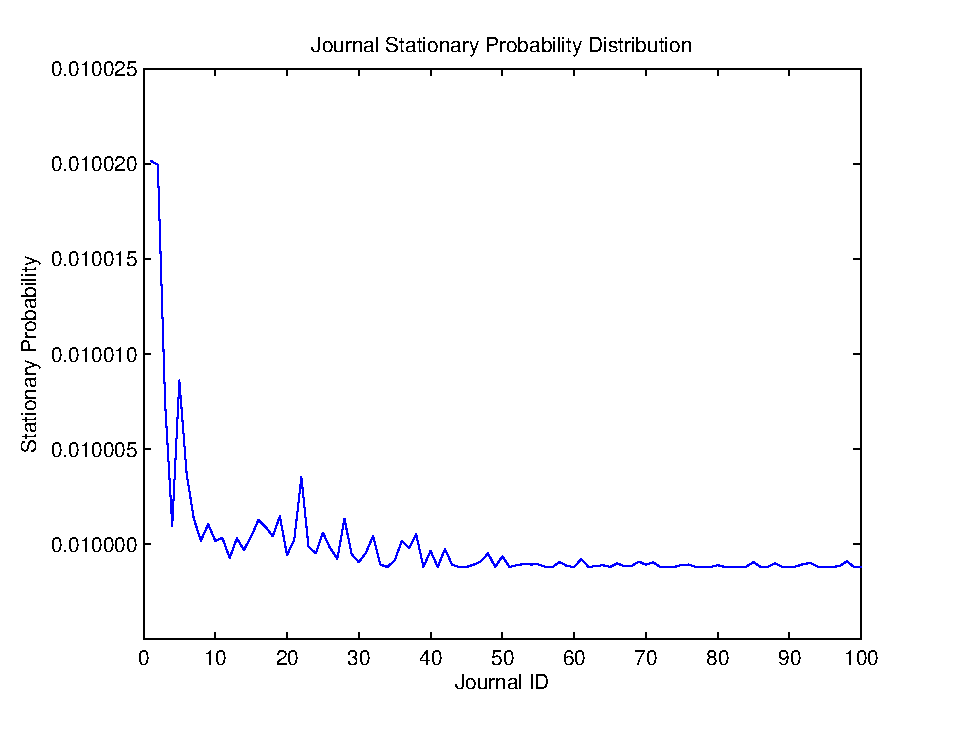
\includegraphics[width=\columnwidth]{journal_dist.eps}}
        \caption{Multirank Stationary Probability Vectors}
        \label{fig:stable}
    \end{figure}

    \begin{figure}[h]
        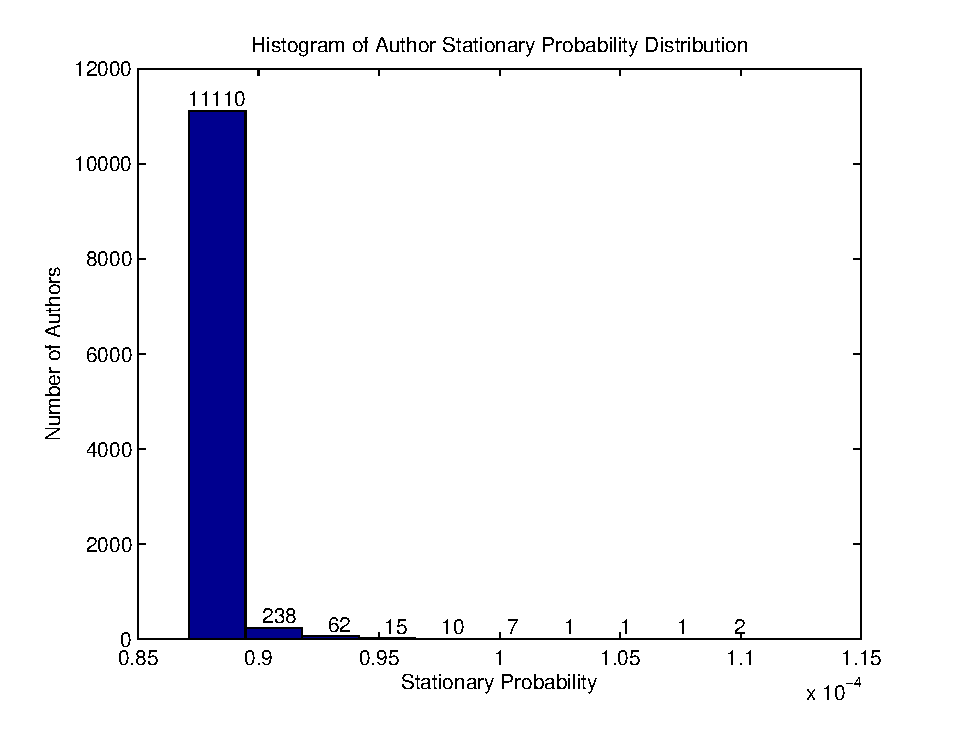
\includegraphics[width=\columnwidth]{author_hist.eps}
        \caption{Histogram of Author Distribution}
        \label{fig:auth_hist}
    \end{figure}

Figure~\ref{fig:stable} shows the plot of the stable probability distribution for journals and authors. From this we can see that there is a clear different in multirank values for authors, but the journal multirank is fairly uniform with a very narrow range of probability values (almost equal to the dangling node probability of $\frac{1}{n=100}$). This hints at two things: firstly, we can take a histogram plot of the author distribution to get a sense of the size of author set to focus on. As seen in Figure~\ref{fig:auth_hist}, only about 100 authors have some significant rank and probably make up a subnetwork of interest. Secondly, the journal relation turns out to be quite insignificant, and thus merely adds complexity to the model. Without the journal relation, Multirank essentially becomes something close to PageRank for authors; but even with journal ranks, which seems nondistinguishing, Multirank has somehow captured the importance of original authorship. We propose some alternative experiments using different relations to explore in the Future Work subsection.



\subsection{Connecting Ranking to Datasets}
In order to obtain conditional probabilities between authors and datasets, we first count the occurences of authors with journals in our underlying data and normalize this to create a joint probability $Pr(Author,Journal)$. This joint can be divided by the learned multiranking for authors $\mathbf{x} = Pr(Author)$ and $\mathbf{y}=Pr(Journal)$ to get conditional probabilities which can be represented as a matrix $M_{A,J}$ of dimension $|A|\times|J|$. To get the connection between author and dataset, we first calculate a linear weighting for datasets. This is calculated for each journal by counting how many times a dataset is connected to the papers published in that journal. $Pr(D=d_1|J=`Plos one')$ is the weighting of dataset 1 for all the datasets connected to papers published in Plos one. A more fine grained weighting would also take into account if the citation to the dataset was a direct citation or required a longer path which requires another run of querying NCBI. Then by multiplying matrix $M_{A,J}$ by the journal-dataset weightings, we obtain a matrix of size $|A|\times|D|$. Each row essentially describes the weighting of datasets and thus a dataset rank for a given author. 

The top three recommended datasets for the top five Multiranked authors is as follows:
    \begin{table}[h]
    \resizebox{\columnwidth}{!}{
    \begin{tabular}{|c|c|ccc|}
    \hline
    \textbf{Original} & \textbf{Author} & \textbf{Rec 1} & \textbf{Rec 2} & \textbf{Rec 3} \\ \hline
    GSE3494 & Bergh, Jonas & GSE2607 & GSE3453 & GSE1378 \\
    GSE3281 & Pollack, Jonathan R & GSE1378 & \textit{GSE3281} & GSE3143 \\
    GSE3281 & Perou, Charles M & GSE1378 & GSE3453 & GSE2990 \\
    GSE2990 & Sotiriou, Christos & GSE3453 & \textit{GSE2990} & GSE1456 \\
    GSE1456 & Pawitan, Yudi & GSE3453 & GSE2990 & \textit{GSE1456} \\ \hline
    \end{tabular}}
    \caption{Dataset Recommendation for Top 5 Multiranked Authors}
    \label{tab:rec}
    \end{table}